% ============================================================================
% Supplementary Material for ICSIS 2026 (EHDS Governance)
% ============================================================================
\documentclass[conference]{IEEEtran}

\usepackage{cite}
\usepackage{amsmath,amssymb,amsfonts}
\usepackage{graphicx}
\usepackage{textcomp}
\usepackage{xcolor}
\usepackage{booktabs}
\usepackage{hyperref}
\usepackage{url}
\usepackage{tikz}
\usetikzlibrary{shapes.geometric, arrows.meta, positioning, fit, backgrounds, calc}

\begin{document}

\title{Supplementary Material:\\Operationalizing the European Health Data Space: A Governance Framework for Privacy-Preserving Cross-Border Health Analytics}

\author{
    \IEEEauthorblockN{Fabio Liberti}
    \IEEEauthorblockA{
        Department of Computer Science\\
        Universitas Mercatorum, Rome, Italy\\
        fabio.liberti@unimercatorum.it\\
        ORCID: 0000-0003-3019-5411
    }
}

\maketitle

\begin{abstract}
This document provides comprehensive supplementary material for the EHDS governance paper, including formal governance algorithm specifications, detailed FHIR/OMOP interoperability components, extended privacy-enhancing technology analysis, Federated Learning algorithm catalogue, infrastructure specifications, and clinical validation details. The open-source reference implementation ($\sim$40K lines, 159 modules) is available at \url{https://github.com/FabioLiberti/FL-EHDS-FLICS2026}.
\end{abstract}

% ============================================================================
\section{Governance Algorithm Specifications}
\label{sec:governance}
% ============================================================================

This section provides formal algorithmic descriptions of all EHDS governance components implemented in the framework.

\subsection{EHDS-Compliant FL Training Procedure}

Algorithm~S1 presents the core training procedure with governance checkpoints integrated at every step.

\begin{figure}[htbp]
\centering
\fbox{\parbox{0.92\columnwidth}{
\small
\textbf{Algorithm S1: EHDS-Compliant FL Training}\\[2pt]
\textbf{Input:} Hospitals $\mathcal{H} = \{h_1, \ldots, h_K\}$, permit $P$, rounds $T$\\
\textbf{Output:} Global model $\theta^{(T)}$\\[3pt]
\textbf{Server executes:}\\
\hspace*{4mm}Initialize $\theta^{(0)}$\\
\hspace*{4mm}\textbf{for} round $t = 1$ to $T$ \textbf{do}\\
\hspace*{8mm}\textit{// Governance check (Layer 1)}\\
\hspace*{8mm}\textbf{if} not ValidatePermit($P$, $t$) \textbf{then abort}\\
\hspace*{8mm}$\mathcal{H}_t \leftarrow$ SelectParticipants($\mathcal{H}$)\\
\hspace*{8mm}\textbf{for each} hospital $h \in \mathcal{H}_t$ \textbf{in parallel do}\\
\hspace*{12mm}$\Delta_h^{(t)}, n_h \leftarrow$ LocalTrain($h$, $\theta^{(t-1)}$)\\
\hspace*{8mm}\textit{// Privacy-preserving aggregation (Layer 2)}\\
\hspace*{8mm}$\theta^{(t)} \leftarrow \theta^{(t-1)} + \frac{1}{\sum n_h} \sum n_h \cdot \Delta_h^{(t)}$\\
\hspace*{8mm}LogCompliance($t$, $\mathcal{H}_t$)\\[3pt]
\textbf{LocalTrain}($h$, $\theta$):\\
\hspace*{4mm}$\mathcal{D}_h \leftarrow$ FilterOptedOut($\mathcal{D}_h$, Registry) \textit{// Art.~71}\\
\hspace*{4mm}$\theta_h \leftarrow \theta$; train $E$ epochs on $\mathcal{D}_h$\\
\hspace*{4mm}$\Delta_h \leftarrow$ ClipGradient($\theta_h - \theta$, $C$) \textit{// DP bound}\\
\hspace*{4mm}\textbf{return} $\Delta_h$, $|\mathcal{D}_h|$
}}
\end{figure}

\subsection{Data Permit Lifecycle Management}

Algorithm~S2 implements the complete permit lifecycle from application through revocation.

\begin{figure}[htbp]
\centering
\fbox{\parbox{0.92\columnwidth}{
\small
\textbf{Algorithm S2: Permit Lifecycle Manager}\\[2pt]
\textbf{Phases:}\\[2pt]
\textit{1. APPLICATION:}\\
\hspace*{4mm}app $\leftarrow$ CreateApplication(purpose, categories, MS)\\
\hspace*{4mm}app.fl\_params $\leftarrow$ (algorithm, rounds, $\varepsilon$-budget)\\
\hspace*{4mm}SubmitToHDAB(app)\\[2pt]
\textit{2. EVALUATION (at HDAB):}\\
\hspace*{4mm}\textbf{if} app.purpose $\notin$ Art53\_Purposes \textbf{then} DENY\\
\hspace*{4mm}\textbf{if} app.$\varepsilon$-budget $<$ MinPrivacyThreshold \textbf{then} DENY\\
\hspace*{4mm}permit $\leftarrow$ ApproveWithConstraints(app, duration, budget)\\[2pt]
\textit{3. EXECUTION:}\\
\hspace*{4mm}\textbf{for each} FL round:\\
\hspace*{8mm}ValidatePermit(permit)\\
\hspace*{8mm}CheckOptOuts(permit.MS)\\
\hspace*{8mm}TrackPrivacyBudget(permit.$\varepsilon$)\\[2pt]
\textit{4. AUDIT:}\\
\hspace*{4mm}GenerateGDPRArt30Report(permit, logs)\\
\hspace*{4mm}ArchiveForRegulatory(permit, 5\_years)
}}
\end{figure}

\subsection{Data Permit Validation}

Algorithm~S3 ensures compliance at every training round.

\begin{figure}[htbp]
\centering
\fbox{\parbox{0.92\columnwidth}{
\small
\textbf{Algorithm S3: Permit Validation (Art.~53)}\\[2pt]
\textbf{Input:} Permit $P$, round $t$, categories $\mathcal{C}$\\
\textbf{Output:} Boolean validity\\[3pt]
\textit{// Temporal validity}\\
\textbf{if} CurrentTime() $>$ $P$.valid\_until \textbf{then}\\
\hspace*{4mm}\textbf{raise} PermitExpiredError\\
\textit{// Purpose alignment (Article 53)}\\
\textbf{if} $P$.purpose $\notin$ AllowedPurposes \textbf{then}\\
\hspace*{4mm}\textbf{raise} PurposeMismatchError\\
\textit{// Category authorization}\\
\textbf{for each} $c \in \mathcal{C}$: \textbf{if} $c \notin P$.categories \textbf{then raise} Error\\
\textit{// Privacy budget check}\\
\textbf{if} $P$.$\varepsilon$\_remaining $< \varepsilon$\_per\_round \textbf{then}\\
\hspace*{4mm}\textbf{raise} PrivacyBudgetExhaustedError\\
\textit{// GDPR Article 30 audit}\\
AuditTrail.log(permit=$P$, round=$t$, categories=$\mathcal{C}$)\\
\textbf{return} True
}}
\end{figure}

\subsection{Article 71 Opt-Out Protocol}

Algorithm~S4 implements citizen opt-out with fine-grained scope support.

\begin{figure}[htbp]
\centering
\fbox{\parbox{0.92\columnwidth}{
\small
\textbf{Algorithm S4: Opt-Out Filtering (Art.~71)}\\[2pt]
\textbf{Input:} Dataset $\mathcal{D}_h$, purpose $p$, categories $\mathcal{C}$\\
\textbf{Output:} Filtered dataset $\mathcal{D}'_h$\\[3pt]
OptOutRecs $\leftarrow$ FetchRegistry(MS) \textit{// LRU-cached, TTL config.}\\
$\mathcal{D}'_h \leftarrow \emptyset$\\
\textbf{for each} record $r \in \mathcal{D}_h$ \textbf{do}\\
\hspace*{4mm}opted\_out $\leftarrow$ False\\
\hspace*{4mm}\textit{// Blanket opt-out check}\\
\hspace*{4mm}\textbf{if} (r.id, ``ALL'') $\in$ OptOutRecs: opted\_out $\leftarrow$ True\\
\hspace*{4mm}\textit{// Purpose-specific}\\
\hspace*{4mm}\textbf{if} (r.id, $p$) $\in$ OptOutRecs: opted\_out $\leftarrow$ True\\
\hspace*{4mm}\textit{// Category-specific}\\
\hspace*{4mm}\textbf{for each} $c \in \mathcal{C}$:\\
\hspace*{8mm}\textbf{if} (r.id, $c$) $\in$ OptOutRecs: opted\_out $\leftarrow$ True\\
\hspace*{4mm}\textbf{if not} opted\_out: $\mathcal{D}'_h \leftarrow \mathcal{D}'_h \cup \{r\}$\\
AuditLog.record(total=$|\mathcal{D}_h|$, filtered=$|\mathcal{D}'_h|$, purpose=$p$)\\
\textbf{return} $\mathcal{D}'_h$
}}
\end{figure}

\textbf{Opt-out granularity}: (1) Blanket---all secondary use; (2) Purpose-specific---e.g., commercial use only; (3) Category-specific---e.g., genomics only. Registry caching: configurable TTL, $<$10ms latency impact, periodic refresh ensures timely propagation.

\subsection{Cross-Border HDAB Consensus Protocol}

Algorithm~S5 coordinates multi-Member State studies.

\begin{figure}[htbp]
\centering
\fbox{\parbox{0.92\columnwidth}{
\small
\textbf{Algorithm S5: Multi-HDAB Coordination}\\[2pt]
\textbf{Input:} Study $S$, Member States $\mathcal{M}$\\
\textbf{Output:} Coordination status, unified permit\\[3pt]
permits $\leftarrow \{\}$\\
\textbf{for each} MS $m \in \mathcal{M}$ \textbf{in parallel do}\\
\hspace*{4mm}$P_m \leftarrow$ SubmitPermitRequest(HDAB$_m$, $S$)\\
\hspace*{4mm}permits[$m$] $\leftarrow$ AwaitApproval($P_m$)\\[2pt]
\textit{// Consensus: ALL HDABs must approve}\\
\textbf{if} $\exists m$: permits[$m$] $=$ DENIED \textbf{then}\\
\hspace*{4mm}NotifyAll($\mathcal{M}$, ``Study denied by'' + $m$)\\
\hspace*{4mm}\textbf{return} DENIED\\[2pt]
\textit{// Harmonize constraints}\\
$P_u$.duration $\leftarrow \min_m$(permits[$m$].duration)\\
$P_u$.$\varepsilon$ $\leftarrow \min_m$(permits[$m$].$\varepsilon$)\\
$P_u$.categories $\leftarrow \bigcap_m$(permits[$m$].categories)\\[2pt]
\textit{// Monitor for mid-study revocation}\\
StartRevocationMonitor($\mathcal{M}$, permits)\\
\textbf{return} APPROVED, $P_u$
}}
\end{figure}

\textbf{Graceful degradation}: If one HDAB revokes mid-study, the coordinator: (1) pauses FL training; (2) notifies all parties; (3) removes the revoking MS's clients; (4) optionally continues with remaining MS if study objectives can be met; (5) logs the event for audit.

\subsection{GDPR Article 30 Audit Trail}

\begin{figure}[htbp]
\centering
\fbox{\parbox{0.92\columnwidth}{
\small
\textbf{Algorithm S6: Audit Trail Persistence}\\[2pt]
\textbf{Input:} FL round context\\[3pt]
record $\leftarrow$ AuditRecord(\\
\hspace*{4mm}timestamp = ISO8601\_UTC(),\\
\hspace*{4mm}permit\_id = current\_permit.id,\\
\hspace*{4mm}purpose = current\_permit.purpose,\\
\hspace*{4mm}participating\_MS = list(active\_clients.MS),\\
\hspace*{4mm}data\_categories = list(accessed\_categories),\\
\hspace*{4mm}privacy\_budget\_consumed = $\varepsilon$\_this\_round,\\
\hspace*{4mm}privacy\_budget\_remaining = $\varepsilon$\_total $-$ $\varepsilon$\_spent,\\
\hspace*{4mm}records\_processed = count\_after\_optout,\\
\hspace*{4mm}records\_excluded\_optout = count\_opted\_out,\\
\hspace*{4mm}model\_metrics = \{accuracy, loss, AUC\},\\
\hspace*{4mm}anomalies = list(detected\_anomalies)\\
)\\
AuditStore.persist(record) \textit{// Append-only, immutable}\\
\textbf{if} record.anomalies: AlertRegulator(record)
}}
\end{figure}

% ============================================================================
\section{FHIR R4 Preprocessing Pipeline}
\label{sec:fhir}
% ============================================================================

\subsection{Data Harmonization}

\begin{figure}[htbp]
\centering
\fbox{\parbox{0.92\columnwidth}{
\small
\textbf{Algorithm S7: FHIR R4 Data Harmonization}\\[2pt]
\textbf{Input:} Raw EHR records $\mathcal{R}$, feature spec $\mathcal{F}$\\
\textbf{Output:} Training tensors $(X, y)$\\[3pt]
\textit{// Stage 1: Format detection}\\
format $\leftarrow$ DetectFormat($\mathcal{R}$)\\
parser $\leftarrow$ GetParser(format) \textit{// HL7v2, CDA, CSV}\\
records $\leftarrow$ parser.parse($\mathcal{R}$)\\[2pt]
\textit{// Stage 2: Terminology mapping}\\
\textbf{for each} $r \in$ records \textbf{do}\\
\hspace*{4mm}$r$.diagnoses $\leftarrow$ MapToICD10($r$.diagnoses)\\
\hspace*{4mm}$r$.medications $\leftarrow$ MapToATC($r$.medications)\\
\hspace*{4mm}$r$.labs $\leftarrow$ MapToLOINC($r$.labs)\\[2pt]
\textit{// Stage 3: FHIR transformation}\\
fhir\_bundle $\leftarrow$ ToFHIR(records)\\
ValidateFHIR(fhir\_bundle) \textit{// Structural + terminology}\\[2pt]
\textit{// Stage 4: ML tensor extraction}\\
$X \leftarrow$ ExtractFeatures(fhir\_bundle, $\mathcal{F}$)\\
$X \leftarrow$ StandardScaler.fit\_transform($X$)\\
$y \leftarrow$ ExtractLabels(fhir\_bundle)\\
\textbf{return} $(X, y)$
}}
\end{figure}

\textbf{Supported FHIR R4 Resources}: Patient, Observation, Condition, MedicationRequest, Procedure, DiagnosticReport.

\textbf{Coding Systems}: SNOMED-CT, LOINC, ICD-10, ATC, UCUM.

\textbf{EHDS Data Categories} (Article~33): Patient Summary, E-Prescription, Laboratory Results, Medical Imaging, Hospital Discharge, Rare Disease.

\subsection{OMOP CDM Integration}

OMOP CDM v5.4 provides an alternative harmonization path for observational research networks (EHDEN, OHDSI).

\textbf{ETL Pipelines}: Transform source EHR to OMOP. \textbf{Vocabulary Mapping}: Standard concepts (SNOMED, ICD10, LOINC, RxNorm). \textbf{Cohort Definitions}: ATLAS-compatible SQL generation. \textbf{Feature Extraction}: FeatureExtraction package for ML-ready datasets.

\textbf{FL Integration}: (1) Each hospital transforms local EHR to OMOP; (2) Feature extraction produces identical schema; (3) FL training proceeds on homogeneous feature spaces across institutions.

% ============================================================================
\section{Extended Interoperability Standards}
\label{sec:interop}
% ============================================================================

\subsection{IHE Integration Profiles}

\textbf{ATNA (Audit Trail and Node Authentication):}
\begin{itemize}
    \item TLS mutual authentication between FL nodes
    \item Syslog audit messages for all data access events (RFC 5424)
    \item Maps directly to GDPR Article~30 record-keeping
\end{itemize}

\textbf{BPPC (Basic Patient Privacy Consents):}
\begin{itemize}
    \item Maps Article~71 opt-out to BPPC consent documents
    \item XDS.b integration for consent document sharing
    \item Consent enforcement at FL training initiation
\end{itemize}

\textbf{XCA (Cross-Community Access):}
\begin{itemize}
    \item Cross-border document query and retrieve
    \item Initiating/Responding Gateway implementation
    \item Patient identity correlation across communities
\end{itemize}

\textbf{PIX/PDQ (Patient Identifier Cross-referencing / Demographics Query):}
\begin{itemize}
    \item Patient matching across institutional boundaries
    \item Pseudonymization-aware identity management
    \item Integration with national eHealth infrastructures
\end{itemize}

\textbf{XUA (Cross-Enterprise User Assertion):}
\begin{itemize}
    \item SAML 2.0 assertions for federated authentication
    \item Role-based access control integration
    \item HDAB authorization token propagation
\end{itemize}

\subsection{Cross-Border Data Exchange}

\textbf{Message Formats}: EHDS Data Permit Exchange Format (JSON-LD), Federated Query Protocol (SPARQL Federation), Model Update Message Format (Protocol Buffers).

\textbf{Security Requirements}: eIDAS-compliant electronic signatures for permits, TLS~1.3 for all cross-border communication, certificate-based node authentication (EU trust framework).

\textbf{Metadata Standards}: DCAT-AP Health extension for dataset cataloging, W3C PROV-O provenance, EMA data quality indicators.

\subsection{Interoperability Architecture}

\begin{figure}[htbp]
\centering
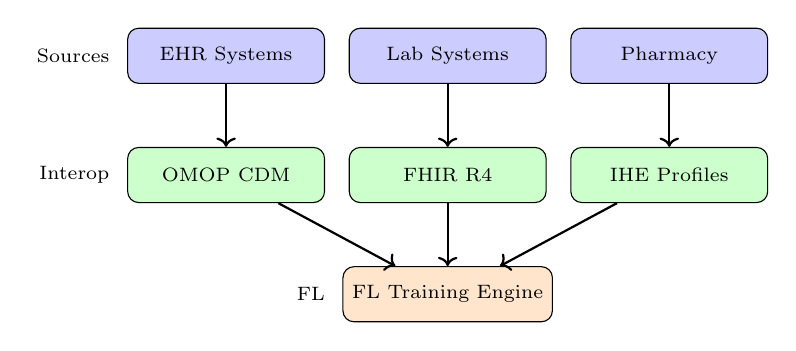
\begin{tikzpicture}[
    node distance=0.8cm,
    box/.style={draw, rounded corners, minimum width=2.5cm, minimum height=0.7cm, font=\scriptsize},
]
\node[box, fill=blue!20] (ehr) {EHR Systems};
\node[box, fill=blue!20, right=0.3cm of ehr] (lab) {Lab Systems};
\node[box, fill=blue!20, right=0.3cm of lab] (pharm) {Pharmacy};
\node[box, fill=green!20, below=0.8cm of lab] (fhir) {FHIR R4};
\node[box, fill=green!20, left=0.3cm of fhir] (omop) {OMOP CDM};
\node[box, fill=green!20, right=0.3cm of fhir] (ihe) {IHE Profiles};
\node[box, fill=orange!20, below=0.8cm of fhir] (fl) {FL Training Engine};
\node[left=0.1cm of ehr, font=\scriptsize] {Sources};
\node[left=0.1cm of omop, font=\scriptsize] {Interop};
\node[left=0.1cm of fl, font=\scriptsize] {FL};
\draw[->, thick] (ehr) -- (omop);
\draw[->, thick] (lab) -- (fhir);
\draw[->, thick] (pharm) -- (ihe);
\draw[->, thick] (omop) -- (fl);
\draw[->, thick] (fhir) -- (fl);
\draw[->, thick] (ihe) -- (fl);
\end{tikzpicture}
\caption{Interoperability layer integrating heterogeneous data sources for FL training.}
\label{fig:interop}
\end{figure}

% ============================================================================
\section{Privacy-Enhancing Technology Details}
\label{sec:pets}
% ============================================================================

\subsection{Differential Privacy}

\begin{figure}[htbp]
\centering
\fbox{\parbox{0.92\columnwidth}{
\small
\textbf{Algorithm S8: Gaussian DP with R\'enyi Accounting}\\[2pt]
\textbf{Input:} Gradient $\Delta$, clip norm $C$, budget $\varepsilon$, $\delta$\\
\textbf{Output:} Noisy gradient $\tilde{\Delta}$\\[3pt]
$\sigma \leftarrow C \cdot \sqrt{2 \ln(1.25/\delta)} / \varepsilon$\\
\textbf{for each} parameter $w \in \Delta$ \textbf{do}\\
\hspace*{4mm}$\tilde{w} \leftarrow w + \mathcal{N}(0, \sigma^2)$\\[2pt]
\textit{// R\'enyi DP moment accounting}\\
PrivacyAccountant.record\_step($\sigma$, sampling\_rate)\\
$\varepsilon_{spent} \leftarrow$ PrivacyAccountant.get\_epsilon($\delta$)\\
\textbf{if} $\varepsilon_{spent} > \varepsilon_{total}$ \textbf{then}\\
\hspace*{4mm}\textbf{raise} BudgetExhaustedError \textit{// Hard stop}\\
\textbf{return} $\tilde{\Delta}$
}}
\end{figure}

\textbf{R\'enyi DP (RDP)} provides 5--6$\times$ tighter composition bounds for the 20+ rounds typical of EHDS studies. For Gaussian mechanisms with noise scale $\sigma$, the RDP guarantee at order $\alpha$ is $\rho(\alpha) = \alpha/(2\sigma^2)$.

\textbf{Governance implications}: The $\varepsilon$-budget must be specified in the data permit application, approved by the HDAB, and tracked throughout training. Budget exhaustion triggers automatic training termination---preventing ``privacy bankruptcy.''

\subsection{Secure Aggregation}

\begin{figure}[htbp]
\centering
\fbox{\parbox{0.92\columnwidth}{
\small
\textbf{Algorithm S9: Pairwise Masking Protocol}\\[2pt]
\textbf{Input:} Gradients $\{\Delta_1, \ldots, \Delta_K\}$, threshold $t$\\
\textbf{Output:} Aggregate $\Delta_{agg}$\\[3pt]
\textit{// Phase 1: ECDH key exchange}\\
\textbf{for each} pair $(j,k)$:\\
\hspace*{4mm}$s_{jk} \leftarrow$ ECDH($pk_j$, $sk_k$)\\
\hspace*{4mm}$r_{jk} \leftarrow$ HKDF-SHA256($s_{jk}$, round\_id)\\[2pt]
\textit{// Phase 2: Mask gradients}\\
\textbf{for each} client $k$:\\
\hspace*{4mm}$\hat{\Delta}_k \leftarrow \Delta_k + \sum_{j<k} r_{jk} - \sum_{j>k} r_{kj}$\\[2pt]
\textit{// Phase 3: Aggregate (masks cancel)}\\
$\Delta_{agg} \leftarrow \sum_{k} \hat{\Delta}_k = \sum_k \Delta_k$\\[2pt]
\textit{// Dropout: Shamir reconstruction of missing masks}\\
\textbf{if} $|$ActiveClients$| < t$: \textbf{raise} SecureAggError\\
\textbf{return} $\Delta_{agg}$
}}
\end{figure}

\textbf{Security guarantee}: The aggregation server learns only $\Delta_{agg} = \sum_k \Delta_k$, never individual $\Delta_k$. Combined with DP, this provides defense-in-depth: even if the server is compromised, individual hospital contributions remain protected.

\subsection{Byzantine Resilience}

Six defense methods protect model integrity against malicious participants:

\begin{itemize}
    \item \textbf{Krum}: Selects gradient closest to $n{-}f{-}2$ nearest neighbors
    \item \textbf{Multi-Krum}: Selects top-$m$ Krum scores, then averages
    \item \textbf{Trimmed Mean}: Removes $\beta$-fraction extremes per coordinate
    \item \textbf{Coordinate-wise Median}: Robust estimator per dimension
    \item \textbf{Bulyan}: Two-stage: Krum selection + trimmed mean
    \item \textbf{FLTrust}: Server-guided trust using small trusted dataset
\end{itemize}

\textbf{Governance relevance}: In cross-border EHDS federations, Byzantine resilience protects against compromised institutions, ensuring that a malicious or malfunctioning participant in one Member State cannot corrupt the global model used by all others.

% ============================================================================
\section{FL Algorithm Catalogue}
\label{sec:algorithms}
% ============================================================================

The framework implements 17 FL algorithms spanning 2017--2025:

\begin{table}[htbp]
\centering
\caption{Complete FL Algorithm Catalogue}
\label{tab:algo_catalogue}
\small
\begin{tabular}{llll}
\toprule
\textbf{Algorithm} & \textbf{Venue} & \textbf{Category} & \textbf{Key Property} \\
\midrule
FedAvg & AISTATS'17 & Baseline & Weighted avg. \\
FedProx & MLSys'20 & Non-IID & Proximal reg. \\
SCAFFOLD & ICML'20 & Non-IID & Variance red. \\
FedNova & NeurIPS'20 & Non-IID & Normalized avg. \\
FedDyn & ICLR'21 & Non-IID & Dynamic reg. \\
FedAdam & ICLR'21 & Adaptive & Server momentum \\
FedYogi & ICLR'21 & Adaptive & Sparse stability \\
FedAdagrad & ICLR'21 & Adaptive & Grad.\ accum. \\
Ditto & ICML'21 & Personal. & Dual models \\
Per-FedAvg & NeurIPS'20 & Personal. & MAML-based \\
FedLC & ICML'22 & Label skew & Logit calibration \\
FedSAM & ICML'22 & Generalize & Flat minima \\
FedDecorr & ICLR'23 & Represent. & Decorrelation \\
FedSpeed & ICLR'23 & Efficiency & Fewer rounds \\
FedExP & ICLR'23 & Server-side & POCS step size \\
\textbf{FedLESAM} & \textbf{ICML'24} & \textbf{Generalize} & \textbf{Global SAM} \\
\textbf{HPFL} & \textbf{ICLR'25} & \textbf{Personal.} & \textbf{Local classif.} \\
\bottomrule
\end{tabular}

\vspace{1mm}
\footnotesize{\textbf{Bold}: 2024--2025 additions. All implemented in the open-source reference.}
\end{table}

\subsection{Algorithm Selection for EHDS Governance}

Table~\ref{tab:algo_selection} maps governance scenarios to recommended algorithms.

\begin{table}[htbp]
\centering
\caption{Algorithm Selection for EHDS Governance Scenarios}
\label{tab:algo_selection}
\small
\begin{tabular}{p{2.6cm}p{1.8cm}p{2.8cm}}
\toprule
\textbf{Governance Scenario} & \textbf{Algorithm} & \textbf{Rationale} \\
\midrule
Homogeneous MS & FedAvg & Simple, auditable \\
Heterogeneous MS & SCAFFOLD & Handles data skew \\
Privacy-critical permits & FedAvg + DP & Best-studied bounds \\
Label-imbalanced data & FedLC & Class calibration \\
Per-hospital needs & HPFL & Local classifiers \\
Comm.-constrained & FedSpeed & Fewer rounds \\
Rapid deployment & FedExP & Server-side only \\
\bottomrule
\end{tabular}

\vspace{1mm}
\footnotesize{MS = Member States. Algorithm choice should be specified in the data permit application for HDAB evaluation.}
\end{table}

% ============================================================================
\section{Infrastructure and Deployment}
\label{sec:infrastructure}
% ============================================================================

\subsection{Communication Layer}

\textbf{gRPC}: Bidirectional streaming, Protocol Buffers serialization (30\% bandwidth reduction vs.\ JSON), HTTP/2 multiplexing. Suitable for data center deployments with low-latency requirements.

\textbf{WebSocket}: Browser-compatible, firewall-friendly (HTTP upgrade), event-driven. Suitable for edge deployments and browser-based participation.

\textbf{Compression}: GZIP, LZ4, ZSTD, Snappy---configurable per deployment.

\subsection{Orchestration}

\textbf{Kubernetes}: FL clients/aggregators as pods, HPA for elastic scaling, ConfigMaps for hyperparameters, Secrets for HDAB API keys.

\textbf{Ray}: Actor-based FL with automatic fault tolerance, Ray Tune for federated hyperparameter optimization.

\textbf{EHDS-Specific}: Data residency constraints (gradients processed within national boundaries), permit-aware deployment, regional restrictions.

\subsection{Monitoring and Alerting}

\textbf{Prometheus Metrics}: rounds\_total, permits\_validated, privacy\_budget\_remaining, active\_clients, round\_duration, communication\_latency.

\textbf{Governance Alerts}: Privacy budget exhaustion warning, permit expiration alerts, opt-out rate spikes, cross-border consensus failures, model divergence detection.

\subsection{User Interfaces}

\textbf{Streamlit Dashboard} (15 modules): EHDS governance workflow screens, real-time FL monitoring, permit management, dataset exploration, paper experiment runner.

\textbf{Terminal UI} (11 screens): Algorithm configuration, dataset management, Byzantine settings, hierarchical FL, continual learning, multi-task FL, vertical FL, privacy settings, cross-border coordination.

% ============================================================================
\section{Experimental Validation Details}
\label{sec:experiments}
% ============================================================================

\subsection{Datasets}

\textbf{Tabular}:
\begin{itemize}
    \item Heart Disease UCI: 920 patients from 4 international hospitals (Cleveland, Hungarian, Swiss, VA Long Beach). 13 clinical features, binary cardiac diagnosis. Natural non-IID from geographical variation.
    \item Diabetes 130-US: 101,766 encounters from 130 US hospitals. 22 features, binary 30-day readmission ($\sim$11\% positive rate). Partitioned via Dirichlet $\alpha{=}0.5$.
\end{itemize}

\textbf{Imaging} (V2 experiments):
\begin{itemize}
    \item Chest X-ray: 5,860 pediatric radiographs (NORMAL/PNEUMONIA)
    \item Brain Tumor MRI: 3,064 T1-weighted CE slices (3-class)
    \item Skin Cancer: 3,297 dermoscopy images (binary)
\end{itemize}

\subsection{Governance Workflow Executed}

\begin{enumerate}
    \item Permit application: ``scientific research'' (Art.~53(1)(b))
    \item HDAB evaluation: auto-approval with 20-round budget, $\varepsilon{=}10$
    \item Per-round: permit validation + opt-out filtering + DP
    \item FL training: 5 algorithms compared (FedAvg, FedProx, SCAFFOLD, FedNova, Ditto)
    \item Audit trail: 100\% GDPR Art.~30 field coverage
\end{enumerate}

\subsection{Governance Overhead}

\begin{itemize}
    \item Permit validation: $<$50ms/round
    \item Opt-out registry lookup: $<$10ms/round (LRU cached)
    \item Cross-border consensus: $<$200ms for 4-country study
    \item Audit trail write: $<$5ms/round
    \item \textbf{Total governance overhead}: $<$0.3\% of training time
\end{itemize}

\subsection{Reproducibility}

\begin{verbatim}
cd fl-ehds-framework
# Full experiments (7 algo x 5 datasets x 3 seeds)
python -m benchmarks.run_full_experiments
# Quick validation (~1-2h)
python -m benchmarks.run_full_experiments --quick
# Resume after interruption
python -m benchmarks.run_full_experiments --resume
\end{verbatim}

\subsection{Supplementary Experimental Figures}

The following figures from the benchmark suite provide additional insights:

\begin{itemize}
    \item Hospital data distribution showing demographic heterogeneity
    \item Per-client training time variation across hospitals
    \item Client participation matrix over 50 rounds
    \item Gradient norm evolution (convergence indicator)
    \item Communication cost analysis (cumulative)
    \item Learning rate sensitivity ($\eta \in \{0.01, 0.05, 0.1, 0.2, 0.5\}$)
    \item Batch size impact ($\{8, 16, 32, 64, 128\}$)
    \item Per-client accuracy trajectories
\end{itemize}

All figures are available in the repository under \texttt{paper/figures/}.

% ============================================================================
\section{Reference Implementation Summary}
\label{sec:implementation}
% ============================================================================

The open-source codebase ($\sim$40,000 lines, 159 Python modules):

\begin{table}[htbp]
\centering
\caption{Codebase Module Summary}
\small
\begin{tabular}{lrl}
\toprule
\textbf{Module} & \textbf{Files} & \textbf{Key Components} \\
\midrule
core/ & 36+ & FL algorithms, security, governance \\
terminal/ & 15 & CLI with 11 specialized screens \\
dashboard/ & 15 & Streamlit web interface \\
data/ & 7 & FHIR, OMOP, dataset loaders \\
models/ & 3 & ResNet-18, MLP, CNN \\
tests/ & 6 & Governance, DP, config tests \\
benchmarks/ & 2+ & Paper experiment suite \\
docs/ & 6 & Architecture, algorithm docs \\
\bottomrule
\end{tabular}
\end{table}

\textbf{Key implementation components}:
\begin{itemize}
    \item \texttt{core/hdab\_api.py}: 1,900+ lines implementing the complete HDAB governance API including DataPermitApplication, DataPermit, OptOutRecord, HDABServiceSimulator, FLEHDSPermitManager, and CrossBorderHDABCoordinator
    \item \texttt{core/fl\_algorithms.py}: All 17 FL algorithms with metadata
    \item \texttt{core/secure\_aggregation.py}: Pairwise masking with ECDH
    \item \texttt{core/byzantine\_resilience.py}: 6 defense methods + attack simulation
    \item \texttt{core/fhir\_integration.py}: FHIR R4 resources and coding systems
    \item \texttt{dashboard/ehds\_tab.py}: EHDS governance workflow UI
\end{itemize}

\noindent Repository: \url{https://github.com/FabioLiberti/FL-EHDS-FLICS2026}

% ============================================================================
\bibliographystyle{IEEEtran}
\begin{thebibliography}{23}

\bibitem{eu2025ehds}
European Commission, ``Regulation (EU) 2025/327 on the European Health Data Space,'' \textit{Official Journal of the EU}, L 2025/327, Mar. 2025.

\bibitem{ganna2024boost}
A. Ganna, E. Ingelsson, and D. Posthuma, ``The European Health Data Space can be a boost for research beyond borders,'' \textit{Nature Medicine}, vol.~30, pp.~3053--3056, 2024.

\bibitem{staunton2024ethical}
C. Staunton \textit{et al.}, ``Ethical and social reflections on the proposed European Health Data Space,'' \textit{Eur.~J.~Human Genetics}, vol.~32, no.~5, pp.~498--505, 2024.

\bibitem{quinn2024gdpr}
P. Quinn, E. Ellyne, and C. Yao, ``Will the GDPR restrain health data access bodies under the EHDS?'' \textit{Computer Law \& Security Review}, vol.~54, art.~105993, 2024.

\bibitem{tehdas2024ready}
TEHDAS Joint Action, ``Are EU member states ready for the European Health Data Space?'' \textit{Eur.~J.~Public Health}, vol.~34, no.~6, pp.~1102--1108, 2024.

\bibitem{frohlich2025reality}
H. Fr\"ohlich \textit{et al.}, ``Reality check: The aspirations of the EHDS amidst challenges in decentralized data analysis,'' \textit{J.~Med.~Internet Res.}, vol.~27, art.~e76491, 2025.

\bibitem{vandrumpt2025pets}
S. van Drumpt \textit{et al.}, ``Secondary use under the European Health Data Space: Setting the scene and towards a research agenda on privacy-enhancing technologies,'' \textit{Frontiers in Digital Health}, vol.~7, art.~1602101, 2025.

\bibitem{hussein2025interop}
R. Hussein \textit{et al.}, ``Interoperability framework of the EHDS for secondary use: Interactive EIF-based standards compliance toolkit,'' \textit{J.~Med.~Internet Res.}, vol.~27, art.~e69813, 2025.

\bibitem{forster2025journeys}
R. Forster \textit{et al.}, ``User journeys in cross-European secondary use of health data,'' \textit{Eur.~J.~Public Health}, vol.~35, Suppl.~3, pp.~iii18--iii24, 2025.

\bibitem{svingel2025hdab}
L. Svingel \textit{et al.}, ``Shaping the future EHDS: Recommendations for implementation of Health Data Access Bodies,'' \textit{Eur.~J.~Public Health}, vol.~35, Suppl.~3, pp.~iii32--iii38, 2025.

\bibitem{christiansen2025pilot}
C. Christiansen \textit{et al.}, ``Piloting an infrastructure for secondary use of health data: Learnings from the HealthData@EU Pilot,'' \textit{Eur.~J.~Public Health}, vol.~35, Suppl.~3, pp.~iii3--iii4, 2025.

\bibitem{shabani2024ehds}
M. Shabani and P. Borry, ``The European Health Data Space: Challenges and opportunities for health data governance,'' \textit{Eur.~J.~Human Genetics}, vol.~32, no.~8, pp.~891--897, 2024.

\bibitem{ohdsi2019omop}
OHDSI, ``The Book of OHDSI: Observational Health Data Sciences and Informatics,'' 2019.

\bibitem{mcmahan2017communication}
B. McMahan \textit{et al.}, ``Communication-efficient learning of deep networks from decentralized data,'' in \textit{Proc. AISTATS}, pp.~1273--1282, 2017.

\bibitem{kairouz2021advances}
P. Kairouz \textit{et al.}, ``Advances and open problems in federated learning,'' \textit{Found.~Trends Mach.~Learn.}, vol.~14, no.~1--2, pp.~1--210, 2021.

\bibitem{li2020federated}
T. Li \textit{et al.}, ``Federated optimization in heterogeneous networks,'' in \textit{Proc. MLSys}, vol.~2, pp.~429--450, 2020.

\bibitem{zhu2019deep}
L. Zhu, Z. Liu, and S. Han, ``Deep leakage from gradients,'' in \textit{Proc. NeurIPS}, vol.~32, pp.~14774--14784, 2019.

\bibitem{mironov2017renyi}
I. Mironov, ``R\'enyi differential privacy,'' in \textit{Proc. IEEE CSF}, pp.~263--275, 2017.

\bibitem{teo2024systematic}
Z. L. Teo \textit{et al.}, ``Federated machine learning in healthcare: A systematic review,'' \textit{Cell Reports Medicine}, vol.~5, no.~2, art.~101419, 2024.

\bibitem{qu2024fedlesam}
Z. Qu \textit{et al.}, ``FedLESAM: Federated learning with locally estimated sharpness-aware minimization,'' in \textit{Proc. ICML}, PMLR 235, 2024.

\bibitem{chen2025hpfl}
Y. Chen, X. Cao, and L. Sun, ``HPFL: Hot-pluggable federated learning with shared backbone and personalized classifiers,'' in \textit{Proc. ICLR}, 2025.

\bibitem{beutel2023flower}
D. J. Beutel \textit{et al.}, ``Flower: A friendly federated learning research framework,'' \textit{arXiv:2007.14390}, 2023.

\bibitem{nvflare2023}
NVIDIA, ``NVIDIA FLARE: An open-source federated learning platform,'' \textit{GitHub Repository}, 2023.

\end{thebibliography}

\end{document}
